\documentclass[11pt,a4paper]{article}
\usepackage[T1]{fontenc}
\usepackage{lmodern}
\usepackage[latin1]{inputenc}
\usepackage{ngerman}
\usepackage{a4wide}
\usepackage[dvips]{graphicx}
\usepackage{float}
\usepackage{pdflscape}
\restylefloat{figure}
\restylefloat{table}

\usepackage[
a4paper,
pdfauthor={ ACE Projekt Team },
pdftitle={ Projektplan },
pdfcreator={pdftex},
]{hyperref}

\usepackage{sectsty}
\allsectionsfont{\sffamily}

\usepackage{fancyheadings} 
\pagestyle{fancy} 
\lhead{\textsf{\textbf{ACE} \\ \small{a collaborative editor}}}
\chead{}
\rhead{
\parbox[c]{3cm}{
\includegraphics[height=0.875cm,width=3cm]{../../images/logo_BFH.eps}}
\parbox[c]{2.2cm}
{\tiny{\textsf{Berner Fachhochschule \\
Hochschule f�r \\
Technik und Informatik}}}}
\lfoot{}
\cfoot{\textsf{\thepage}}
\rfoot{}
\setlength{\headrulewidth}{0.6pt}
\setlength{\footrulewidth}{0.6pt}
\setlength{\topmargin}{-50pt}
\addtolength{\headheight}{50pt}

\usepackage{colortbl}

\newcommand{\headercol}[2]{\multicolumn{1}{|>{\bfseries\columncolor[gray]{0.82}}p{#1}|}{\textsf{#2}}}
\newcommand{\ace}[0]{\emph{ACE }}



\begin{document}

\begin{titlepage}
\thispagestyle{empty}
  
\includegraphics[height=1.5in]{../images/pix.eps}

  \begin{center}

    {\fontsize{40}{45} \textbf{\textsf{ACE}}} \\
    \textsf{a collaborative editor} \\
        
    \vspace{36pt}
        
    {\huge{\textbf{\textsf{}}}} \\

    \vspace{36pt}

	\textsf{Berne University of Applied Sciences} \\
    \textsf{School of Engineering and Information Technology} \\
    
  \end{center}

  \vfill
  
  \begin{tabular}{ll}
   \hline

   \\

   \multicolumn{1}{>{\bfseries}p{1.5in}}{\textsf{Date:}} &
   \multicolumn{1}{>{}p{4.3in}}{\textsf{08.11.2005}}          \\
   
   \\
   
   \multicolumn{1}{>{\bfseries}p{1.5in}}{\textsf{Version:}}     &   
   \multicolumn{1}{>{}p{4.3in}}{\textsf{0.1}}                 \\

   \\
   
   \multicolumn{1}{>{\bfseries}p{1.5in}}{\textsf{Projectteam:}}                 &
   \multicolumn{1}{>{}p{4.3in}}{\textsf{Mark Bigler (biglm2@hta-bi.bfh.ch)}}  \\
   \multicolumn{1}{>{\bfseries}p{1.5in}}{}                                      &
   \multicolumn{1}{>{}p{4.3in}}{\textsf{Simon Raess (rasss@hta-bi.bfh.ch)}}    \\
   \multicolumn{1}{>{\bfseries}p{1.5in}}{}                                      &
   \multicolumn{1}{>{}p{4.3in}}{\textsf{Lukas Zbinden (zbinl@hta-bi.bfh.ch)}} \\   
   
   \\
   
   \multicolumn{1}{>{\bfseries}p{1.5in}}{\textsf{Receivers:}}                       &
   \multicolumn{1}{>{}p{4.3in}}{\textsf{Jean-Paul Dubois (doj@hta-bi.bfh.ch)}}       \\
   \multicolumn{1}{>{\bfseries}p{1.5in}}{}                                          &
   \multicolumn{1}{>{}p{4.3in}}{\textsf{Claude Fuhrer (frc@hta-bi.bfh.ch)}}       \\

   \\
   
   \multicolumn{1}{>{\bfseries}p{1.5in}}{\textsf{Location:}}               &   
   \multicolumn{1}{>{}p{4.3in}}{\textsf{Subversion Repository}} \\

   \\  
   
   \hline
  \end{tabular}

\end{titlepage}

\newpage

\tableofcontents
\newpage
\listoftables
\listoffigures
\newpage

\section*{Versionskontrolle}

\begin{table}[!h]
 \begin{tabular}{|l|l|l|l|}
  \hline
  \headercol{0.6in}{Version}         & 
  \headercol{0.8in}{Datum}           &
  \headercol{1.2in}{Verantwortlich}  & 
  \headercol{2.8in}{Bemerkungen}     \\
  \hline
  0.1         & 15.03.2005  & rasss           &  Erste Version \\
  \hline
  0.2         & 22.03.2005  & rasss zbinl     &  �berarbeitung \\
  \hline
  0.3         & 30.03.2005  & zbinl           &  Projektspezifisches Vorgehensmodell \\
  \hline
  0.4         & 30.03.2005  & rasss zbinl     &  �berarbeitung Punkte 2, 3 und 4 \\
  \hline
  0.5         & 05.04.2005  & zbinl           &  �berarbeitung Appendix A.1 \\
  \hline
  0.6         & 06.04.2005  & zbinl           &  Anpassungen Punkte 2, 3 und 4 \\
  \hline
  0.7         & 06.04.2005  & Projektteam     &  Review \\
  \hline
  0.8         & 13.04.2005  & Projektteam     &  Letzte Anpassungen \\
  \hline
  1.0         & 13.04.2005  & Projektteam     &  Freigabe \\
  \hline
 \end{tabular}
 \caption{Versionskontrolle}
 \label{Versionskontrolle}
\end{table}

\begin{table}[!h]
 \begin{tabular}{|l|l|l|l|l|}
  \hline
  \headercol{0.9in}{}            & 
  \headercol{0.9in}{Stelle}      & 
  \headercol{0.8in}{Datum}       & 
  \headercol{0.6in}{Visum}       & 
  \headercol{2.0in}{Bemerkungen} \\
  \hline
  \textbf{Freigegeben}   & Projektteam &       &       &             \\
  \hline
  \textbf{Genehmigt}     &             &       &       &             \\
  \hline
 \end{tabular}
 \caption{Pr�fung/Genehmigung}
 \label{Pr�fung/Genehmigung}
\end{table}

\newpage


\section{Einleitung}
\subsection{Zweck des Dokumentes}
Der Projektplan enth�lt die Planung und Organisation des gesamten Projekts und erg�nzt das Projekthandbuch als Handlungsgrundlage. Der Projektplan wird fortlaufend nachgef�hrt und verfeinert.


\section{Projektorganisation}


\section{Projektablauf}
Der Projektablauf beschreibt die Ergebnisstruktur des \ace Projektes und darauf aufbauend die ablaufoganisatorischen Gegebenheiten.


\subsection{Ergebnisstruktur}
Alle Ergebnisse, die zum jeweiligen Planungsstand bekannt sind, werden identifiziert und in ihrer Abh�ngigkeit (Struktur) untereinander festgelegt. Dieser Abschnitt enth�lt sowohl die als Vertragsbestandteil festgelegten Ergebnisse als auch die projekinternen Ergebnisse.

\begin{figure}[H]
 \begin{center}
  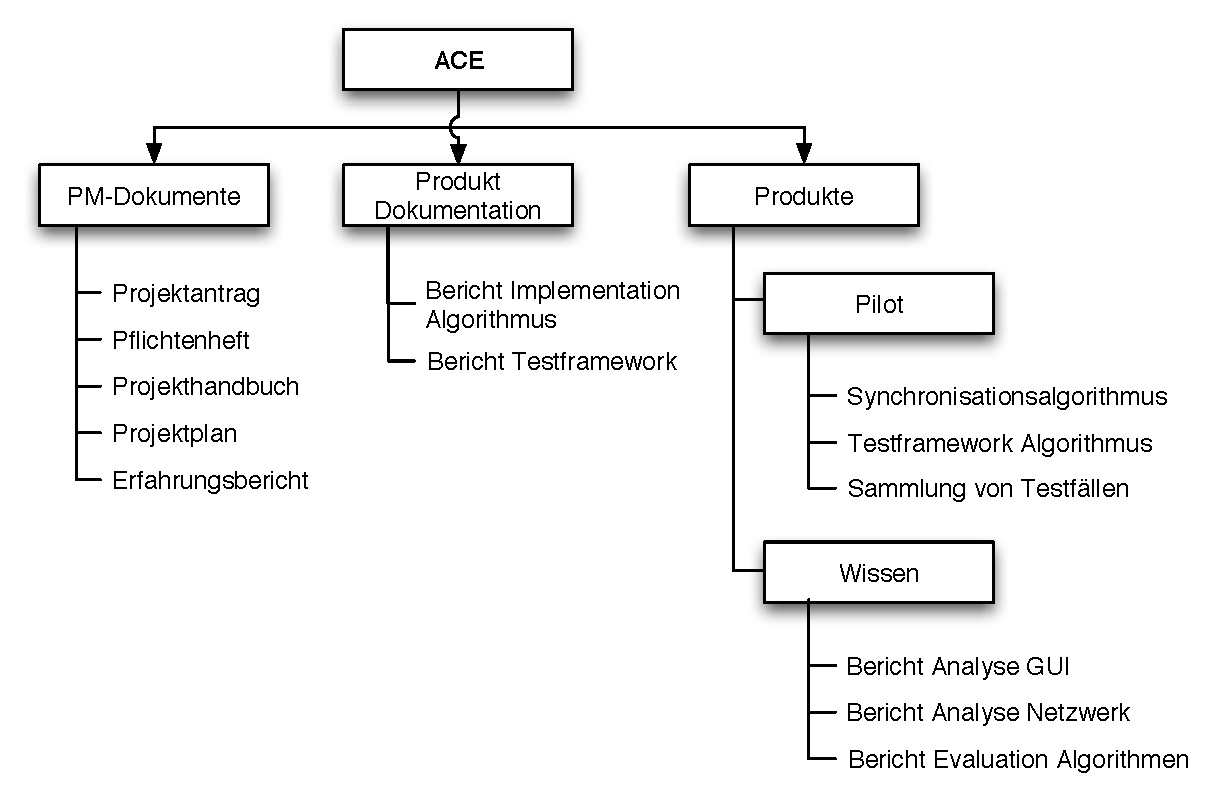
\includegraphics[width=5.5in,height=3.28in]{../../images/ergebnisstrukturplan.eps}
 \end{center}
 \caption{Ergebnisstrukturplan}
 \label{Ergebnisstrukturplan}
\end{figure}

\newpage
\begin{landscape}
\subsection{Ablauforganisation}
 \begin{figure}[H]
  \includegraphics[width=20cm]{../../images/projektplan.eps}
  \caption{Gantt Chart}
  \label{Gantt Chart}
 \end{figure}
\end{landscape}
\newpage

\subsection{Workpackages}

\begin{table}[H]
 \begin{tabular}{|l|l|l|l|}
  \hline
    \multicolumn{3}{|>{\columncolor[gray]{0.82}}p{5.85in}|}{\bfseries{\textsf{Work Package: Infrastruktur}}} \\
  \hline
    \multicolumn{1}{|p{1in}|}{\bfseries{\textsf{Autor}}} &
    \multicolumn{2}{|p{4.5in}|}{Projektteam} \\
  \hline
    \multicolumn{1}{|p{1in}|}{\bfseries{\textsf{Datum}}} &
    \multicolumn{2}{|p{4.5in}|}{29.3.2005} \\
  \hline
    \multicolumn{1}{|p{1in}|}{\bfseries{\textsf{Input}}} &
    \multicolumn{2}{|p{4.5in}|}{} \\
  \hline
    \multicolumn{1}{|p{1in}|}{\bfseries{\textsf{Output}}} &
    \multicolumn{2}{|p{4.5in}|}{Entwicklungsumgebung} \\
    \multicolumn{1}{|p{1in}|}{} &
    \multicolumn{2}{|p{4.5in}|}{Projekt Server} \\
    \multicolumn{1}{|p{1in}|}{} &
    \multicolumn{2}{|p{4.5in}|}{Projekt Website} \\
  \hline
   \multicolumn{1}{|p{1in}|}{\bfseries{\textsf{Skills}}} &
   \multicolumn{2}{|p{4.5in}|}{Installationserfahrung Subversion, Trac, Kalender} \\
  \hline
   \multicolumn{1}{|p{1in}|}{\bfseries{\textsf{Resources}}} &
   \multicolumn{2}{|p{4.5in}|}{Hardware und Software f�r Arbeitspl�tze} \\
   \multicolumn{1}{|p{1in}|}{} &
   \multicolumn{2}{|p{4.5in}|}{Zugriff Projektserver} \\
    
  \hline \hline
    \multicolumn{1}{|>{\columncolor[gray]{0.82}}p{1in}|}{} &
    \multicolumn{1}{|>{\columncolor[gray]{0.82}}p{3.5in}|}{\bfseries{\textsf{Beschreibung}}} &
    \multicolumn{1}{|>{\columncolor[gray]{0.82}}p{1in}|}{\bfseries{\textsf{Aufwand}}} \\
  \hline
    \multicolumn{1}{|p{1in}|}{\bfseries{\textsf{Aktivit�ten}}} &
    \multicolumn{1}{|p{3.5in}|}{PC installieren} &
    \multicolumn{1}{|p{1in}|}{2 Tage} \\
    \multicolumn{1}{|p{1in}|}{} &
    \multicolumn{1}{|p{3.5in}|}{Projekt Server installieren (Subversion, Trac, Kalender)} &
    \multicolumn{1}{|p{1in}|}{1 Tag} \\
    \multicolumn{1}{|p{1in}|}{} &
    \multicolumn{1}{|p{3.5in}|}{Projekt Website einrichten} &
    \multicolumn{1}{|p{1in}|}{1 Tag} \\    
  \hline
    \multicolumn{1}{|p{1in}|}{\bfseries{\textsf{QA}}} &
    \multicolumn{1}{|p{3.5in}|}{} &
    \multicolumn{1}{|p{1in}|}{} \\
  \hline \hline
    \multicolumn{1}{|p{1in}|}{\bfseries{\textsf{Total}}} &
    \multicolumn{1}{|p{3.5in}|}{} &
    \multicolumn{1}{|p{1in}|}{4 Tage} \\
  \hline
 \end{tabular}
 \caption{Workpackage Infrastruktur}
 \label{Workpackage Infrastruktur}
\end{table}


\begin{table}[H]
 \begin{tabular}{|l|l|l|l|}
  \hline
  \multicolumn{3}{|>{\columncolor[gray]{0.82}}p{5.85in}|}{\bfseries{\textsf{Work Package: Projektantrag}}} \\
  \hline
    \multicolumn{1}{|p{1in}|}{\bfseries{\textsf{Autor}}} &
    \multicolumn{2}{|p{4.5in}|}{Projektteam} \\
  \hline
    \multicolumn{1}{|p{1in}|}{\bfseries{\textsf{Datum}}} &
    \multicolumn{2}{|p{4.5in}|}{5.4.2005} \\
  \hline
    \multicolumn{1}{|p{1in}|}{\bfseries{\textsf{Input}}} &
    \multicolumn{2}{|p{4.5in}|}{einsatzbereite Infrastruktur} \\
  \hline
    \multicolumn{1}{|p{1in}|}{\bfseries{\textsf{Output}}} &
    \multicolumn{2}{|p{4.5in}|}{Projektantrag} \\
  \hline
   \multicolumn{1}{|p{1in}|}{\bfseries{\textsf{Skills}}} &
   \multicolumn{2}{|p{4.5in}|}{Know-How Projektf�hrung} \\
  \hline
   \multicolumn{1}{|p{1in}|}{\bfseries{\textsf{Resources}}} &
   \multicolumn{2}{|p{4.5in}|}{Projektarbeitspl�tze} \\

  \hline \hline
    \multicolumn{1}{|>{\columncolor[gray]{0.82}}p{1in}|}{} &
    \multicolumn{1}{|>{\columncolor[gray]{0.82}}p{3.5in}|}{\bfseries{\textsf{Beschreibung}}} &
    \multicolumn{1}{|>{\columncolor[gray]{0.82}}p{1in}|}{\bfseries{\textsf{Aufwand}}} \\
  \hline
    \multicolumn{1}{|p{1in}|}{\bfseries{\textsf{Aktivit�ten}}} &
    \multicolumn{1}{|p{3.5in}|}{Besprechung Projektidee} &
    \multicolumn{1}{|p{1in}|}{0.5 Tage} \\    
    \multicolumn{1}{|p{1in}|}{} &
    \multicolumn{1}{|p{3.5in}|}{Verfassen Projektantrag} &
    \multicolumn{1}{|p{1in}|}{2.5 Tage} \\
    \multicolumn{1}{|p{1in}|}{} &
    \multicolumn{1}{|p{3.5in}|}{Korrekturen nach Review} &
    \multicolumn{1}{|p{1in}|}{1 Tag} \\
  \hline
    \multicolumn{1}{|p{1in}|}{\bfseries{\textsf{QA}}} &
    \multicolumn{1}{|p{3.5in}|}{Review durch Projektteam} &
    \multicolumn{1}{|p{1in}|}{1 Tage} \\
  \hline \hline
    \multicolumn{1}{|p{1in}|}{\bfseries{\textsf{Total}}} &
    \multicolumn{1}{|p{3.5in}|}{} &
    \multicolumn{1}{|p{1in}|}{5 Tage} \\
  \hline
 \end{tabular}
 \caption{Workpackage Projektantrag}
 \label{Workpackage Projektantrag}
\end{table}

\documentclass[11pt,a4paper]{article}
\usepackage[T1]{fontenc}
\usepackage{lmodern}
\usepackage[latin1]{inputenc}
\usepackage{ngerman}
\usepackage{a4wide}
\usepackage[dvips]{graphicx}

\usepackage[
pdfauthor={ACE Projekt Team},
pdftitle={Pflichtenheft},
pdfcreator={pdftex},
]{hyperref}

\usepackage{sectsty}
\allsectionsfont{\sffamily}

\usepackage{fancyheadings} 
\pagestyle{fancy} 
\lhead{\textsf{\textbf{ACE} \\ \small{a collaborative editor}}}
\chead{}
\rhead{
\parbox[c]{3cm}{
\includegraphics[height=0.875cm,width=3cm]{../../images/logo_BFH.eps}}
\parbox[c]{2.2cm}
{\tiny{\textsf{Berner Fachhochschule \\
Hochschule f�r \\
Technik und Informatik}}}}
\lfoot{}
\cfoot{\textsf{\thepage}}
\rfoot{}
\setlength{\headrulewidth}{0.6pt}
\setlength{\footrulewidth}{0.6pt}
\setlength{\topmargin}{-50pt}
\addtolength{\headheight}{50pt}

\usepackage{colortbl}

\newcommand{\headercol}[2]{\multicolumn{1}{|>{\bfseries\columncolor[gray]{0.82}}p{#1}|}{\textsf{#2}}}
\newcommand{\ace}[0]{\emph{ACE }}



\begin{document}

\begin{titlepage}
\thispagestyle{empty}
  
\includegraphics[height=1.5in]{../images/pix.eps}

  \begin{center}

    {\fontsize{40}{45} \textbf{\textsf{ACE}}} \\
    \textsf{a collaborative editor} \\
        
    \vspace{36pt}
        
    {\huge{\textbf{\textsf{}}}} \\

    \vspace{36pt}

	\textsf{Berne University of Applied Sciences} \\
    \textsf{School of Engineering and Information Technology} \\
    
  \end{center}

  \vfill
  
  \begin{tabular}{ll}
   \hline

   \\

   \multicolumn{1}{>{\bfseries}p{1.5in}}{\textsf{Date:}} &
   \multicolumn{1}{>{}p{4.3in}}{\textsf{08.11.2005}}          \\
   
   \\
   
   \multicolumn{1}{>{\bfseries}p{1.5in}}{\textsf{Version:}}     &   
   \multicolumn{1}{>{}p{4.3in}}{\textsf{0.1}}                 \\

   \\
   
   \multicolumn{1}{>{\bfseries}p{1.5in}}{\textsf{Projectteam:}}                 &
   \multicolumn{1}{>{}p{4.3in}}{\textsf{Mark Bigler (biglm2@hta-bi.bfh.ch)}}  \\
   \multicolumn{1}{>{\bfseries}p{1.5in}}{}                                      &
   \multicolumn{1}{>{}p{4.3in}}{\textsf{Simon Raess (rasss@hta-bi.bfh.ch)}}    \\
   \multicolumn{1}{>{\bfseries}p{1.5in}}{}                                      &
   \multicolumn{1}{>{}p{4.3in}}{\textsf{Lukas Zbinden (zbinl@hta-bi.bfh.ch)}} \\   
   
   \\
   
   \multicolumn{1}{>{\bfseries}p{1.5in}}{\textsf{Receivers:}}                       &
   \multicolumn{1}{>{}p{4.3in}}{\textsf{Jean-Paul Dubois (doj@hta-bi.bfh.ch)}}       \\
   \multicolumn{1}{>{\bfseries}p{1.5in}}{}                                          &
   \multicolumn{1}{>{}p{4.3in}}{\textsf{Claude Fuhrer (frc@hta-bi.bfh.ch)}}       \\

   \\
   
   \multicolumn{1}{>{\bfseries}p{1.5in}}{\textsf{Location:}}               &   
   \multicolumn{1}{>{}p{4.3in}}{\textsf{Subversion Repository}} \\

   \\  
   
   \hline
  \end{tabular}

\end{titlepage}

\newpage

\tableofcontents
\newpage

\listoftables
\listoffigures
\newpage

\section*{Versionskontrolle}

\begin{table}[!h]
 \begin{tabular}{|l|l|l|l|}
  \hline
  \headercol{0.6in}{Version}         & 
  \headercol{0.8in}{Datum}           &
  \headercol{1.2in}{Verantwortlich}  & 
  \headercol{2.8in}{Bemerkungen}     \\
  \hline
  0.1         & 15.03.2005  & rasss           &  Erste Version \\
  \hline
  0.2         & 22.03.2005  & rasss zbinl     &  �berarbeitung \\
  \hline
  0.3         & 30.03.2005  & zbinl           &  Projektspezifisches Vorgehensmodell \\
  \hline
  0.4         & 30.03.2005  & rasss zbinl     &  �berarbeitung Punkte 2, 3 und 4 \\
  \hline
  0.5         & 05.04.2005  & zbinl           &  �berarbeitung Appendix A.1 \\
  \hline
  0.6         & 06.04.2005  & zbinl           &  Anpassungen Punkte 2, 3 und 4 \\
  \hline
  0.7         & 06.04.2005  & Projektteam     &  Review \\
  \hline
  0.8         & 13.04.2005  & Projektteam     &  Letzte Anpassungen \\
  \hline
  1.0         & 13.04.2005  & Projektteam     &  Freigabe \\
  \hline
 \end{tabular}
 \caption{Versionskontrolle}
 \label{Versionskontrolle}
\end{table}

\begin{table}[!h]
 \begin{tabular}{|l|l|l|l|l|}
  \hline
  \headercol{0.9in}{}            & 
  \headercol{0.9in}{Stelle}      & 
  \headercol{0.8in}{Datum}       & 
  \headercol{0.6in}{Visum}       & 
  \headercol{2.0in}{Bemerkungen} \\
  \hline
  \textbf{Freigegeben}   & Projektteam &       &       &             \\
  \hline
  \textbf{Genehmigt}     &             &       &       &             \\
  \hline
 \end{tabular}
 \caption{Pr�fung/Genehmigung}
 \label{Pr�fung/Genehmigung}
\end{table}

\newpage


\section{Einleitung}
Im Projekt \ace soll ein kollaborativer, plattformunabh�ngiger Editor entwickelt werden. Diese Applikation erm�glicht mehreren Personen, ein Textdokument gemeinsam zu bearbeiten. Dabei arbeitet jede Person mit dem Editor an einem eigenen Computer. Alle Teilnehmer sind �ber ein Netzwerk verbunden und sehen jederzeit den gleichen Dokumentinhalt. Wenn jemand der Gruppe eine �nderung im Dokument vornimmt, wird dies in Echtzeit und synchron allen anderen Benutzern angezeigt. Jeder Benutzer hat dadurch den �berblick �ber alle �nderungen im Dokument. Dieser Editor erm�glicht zum Beispiel ein gemeinsames Brainstorming von mehreren Personen, welche sich an verschiedenen Orten befinden. 

\subsection{Zweck des Dokumentes}
Das vorliegende Dokument beschreibt die Ziele, welche mit der angestrebten L�sung zu erreichen sind sowie die Anforderungen an das in der Semesterarbeit zu erstellende System.


\section{Ausgangslage}
Das gemeinsame Entwerfen eines elektronischen Dokumentes (z.B. Textdatei), wobei jeder Beteiligte mit seinem eigenen Computer arbeitet, ist noch praktisch unbekannt. Diese Technologie birgt ein grosses Anwendungspotenzial. Der zu entwickelnde Editor \ace soll komplett neuartige und effiziente Editier-M�glichkeiten bieten und dadurch neue Wege der Zusammenarbeit er�ffnen. Bis heute existiert keine marktreife, plattformunabh�ngige Applikation dieser Art.


\section{Ist-Zustand}
Die dem kollaborativen Editor zugrunde liegende Theorie entstammt aus dem Forschungsgebiet der "'Computer Supported Cooperative Work - CSCW"'. Applikationen aus diesem Bereich werden auch als "'Groupware"' bezeichnet. Seit Mitte der 90er Jahren sind zahlreiche Forschungsarbeiten geschrieben worden. Die meisten davon beinhalten theoretische �berlegungen, so zum Beispiel mathematische Beschreibungen oder Beweise zu Synchronisationsalgorithmen. Viel Theoriewissen wurde erarbeitet. Dieses Know-How soll nun in die konkrete Implementation eines kollaborativen Editors einfliessen um daraus eine hochentwickelte, konkurrenzf�hige Applikation auf den Markt zu bringen. 


\section{Ziele}
In der Semesterarbeit soll die Basis gelegt werden f�r die Implementation eines kollaborativen und plattformunabh�ngigen Texteditors im Rahmen der Diplomarbeit.

 \begin{table}[!ht]
  \begin{tabular}{|l|c|}
   \hline
   \headercol{4.5in}{Beschreibung}                              & \headercol{1in}{Priorit�t}  \\
   \hline
    Aufbau von Knowhow                                          &        1                    \\
    Evaluation bestehender Algorithmen                          &        1                    \\
    Implementation Algorithmus                                  &        1                    \\
    Testframework f�r Algorithmus                               &        1                    \\
    Konzept GUI                                                 &        2                    \\
    Konzept Netzwerk/Kommunikation                              &        2                    \\
    User Stories f�r kollaborativen Texteditor                  &        3                    \\
   \hline
  \end{tabular}
  \caption{Projektziele}
  \label{Projektziele}
 \end{table}

\subsection{Aufbau von Knowhow}
Es geht darum, ein fundiertes Basiswissen im Bereich des CSCW aufzubauen. Das Ziel ist, eine �bersicht �ber den aktuellen Forschungsstand und �ber die wichtigsten Errungenschaften in diesem Gebiet zu gewinnen. Das angeeignete Know-How soll beim Evaluieren der bestehenden Synchronisationsalgorithmen zum tieferen Verst�ndnis beitragen und ein sachgerechtes Beurteilen erm�glichen.

\subsection{Evaluation bestehender Algorithmen}
Die Forschung hat seit anfangs der 90er Jahre zahlreiche Synchronisations-Algorithmen hervorgebracht. Das Ziel ist eine �bersicht �ber die bestehenden Algorithmen zu erabeiten. Jeder evaluierte Algorithmus soll prinzipiell verstanden werden. Die �bersicht soll Vor- und Nachteile aufzeigen und es erm�glichen, den am besten geeigneten Algorithmus f�r einen kollaborativen Texteditor zu bestimmen.

\subsection{Implementation Algorithmus}
Nach Evaluation der Algorithmen soll einer oder eventuell mehrere implementiert werden. Die Implementation des Algorithmus wird mit dem Testframework gepr�ft.

\subsection{Testframework f�r Algorithmus}
Parallel zur Entwicklung des Synchronisationsalgorithmus soll ein Testframework erstellt werden. Dieses erm�glicht das sorgf�lltige Austesten des Algorithmus mit verschiedenen, klar definierbaren Abl�ufen.

\subsection{Konzept GUI}
In erster Linie soll eine Evaluation von Textkomponenten in Java erfolgen. Das Ziel ist herauszufinden, welche sich am besten f�r einen kollaborativen Texteditor eignen. Es muss m�glich sein, verschiedene Benutzer respektive deren Aktionen in einer Textkomponente darzustellen. 

\subsection{Konzept Netzwerk/Kommunikation}
Zwei Themen m�ssen erarbeitet werden: Das dynamische Auffinden aller vorhandenen Instanzen des Editors in einem Netzwerk sowie der Nachrichtenaustausch zwischen den Instanzen. Es sollen die in diesem Themengebiet vorhandenen Technologien studiert werden. Daraus entsteht ein f�r einen kollaborativen Texteditor angepasstes Konzept. 

\subsection{User Stories f�r kollaborativen Texteditor}
Das Ziel ist, eine Sammlung von User Stories (Anwendungsm�glichkeiten aus Sicht des Benutzers) f�r einen kollaborativen Texteditor zu erstellen. Diese Sammlung bildet dann eine Ideen-Grundlage f�r die Implementation von Funktionen des in der Diplomarbeit zu entwickelnden Texteditors.


\section{Nicht-Ziele}

 \begin{table}[!ht]
  \begin{tabular}{|l|c|}
   \hline
   \headercol{4.5in}{Beschreibung}                              \\
   \hline
    Ausarbeiten von Sicherheitsaspekten                         \\
    Prototyp kollaborativer Text-Editor                         \\
   \hline
  \end{tabular}
  \caption{Nicht-Ziele}
  \label{Nicht-Projektziele}
 \end{table}

\subsection{Ausarbeiten von Sicherheitsaspekten}
Es ist nicht das Ziel Sicherheitsaspekte wie Authentifikation, Authorisierung und Verschl�sselung zu ber�cksichtigen. Es wird auch kein Konzept erstellt. 

\subsection{Prototyp kollaborativer Text-Editor}
Im Rahmen der Semesterarbeit soll kein Prototyp eines kollaborativen Editors entstehen.


\section{Anforderungen}
\subsection{Architektur}
Die Architektur wird basierend auf dem Peer-to-Peer Modell entwickelt. Die Applikation soll dadurch ohne einen zentralen Server funktionieren.

\subsection{Schnittstellen}
Durch die Offenlegung des internen Kommunikations-Protokolls von \ace haben andere Applikationsentwickler die M�glichkeit, direkt mit dem Editor zu kommunizieren. Dadurch entstehen beliebige Erweiterungsm�glichkeiten mit dem kollaborativen Texteditor.

\end{document}

\begin{table}[H]
 \begin{tabular}{|l|l|l|l|}
  \hline
   \multicolumn{3}{|>{\columncolor[gray]{0.82}}p{5.85in}|}{\bfseries{\textsf{Work Package: Projekthandbuch}}} \\
  \hline
   \multicolumn{1}{|p{1in}|}{\bfseries{\textsf{Autor}}} &
   \multicolumn{2}{|p{4.5in}|}{Projektteam} \\
  \hline
   \multicolumn{1}{|p{1in}|}{\bfseries{\textsf{Datum}}} &
   \multicolumn{2}{|p{4.5in}|}{29.3.2005} \\
  \hline
   \multicolumn{1}{|p{1in}|}{\bfseries{\textsf{Input}}} &
   \multicolumn{2}{|p{4.5in}|}{Projektantrag} \\
  \hline
   \multicolumn{1}{|p{1in}|}{\bfseries{\textsf{Output}}} &
   \multicolumn{2}{|p{4.5in}|}{Projekthandbuch} \\
  \hline
   \multicolumn{1}{|p{1in}|}{\bfseries{\textsf{Skills}}} &
   \multicolumn{2}{|p{4.5in}|}{Know-How Projektf�hrung} \\
  \hline
   \multicolumn{1}{|p{1in}|}{\bfseries{\textsf{Resources}}} &
   \multicolumn{2}{|p{4.5in}|}{Arbeitspl�tze} \\
   \multicolumn{1}{|p{1in}|}{} &
   \multicolumn{2}{|p{4.5in}|}{Hermes Dokumentation} \\

  \hline \hline
   \multicolumn{1}{|>{\columncolor[gray]{0.82}}p{1in}|}{} &
   \multicolumn{1}{|>{\columncolor[gray]{0.82}}p{3.5in}|}{\bfseries{\textsf{Beschreibung}}} &
   \multicolumn{1}{|>{\columncolor[gray]{0.82}}p{1in}|}{\bfseries{\textsf{Aufwand}}} \\
  \hline
   \multicolumn{1}{|p{1in}|}{\bfseries{\textsf{Aktivit�ten}}} &
   \multicolumn{1}{|p{3.5in}|}{Besprechung Ziele, Ergebnisse, Entscheidungspunkte} &
   \multicolumn{1}{|p{1in}|}{0.5 Tage} \\  
   \multicolumn{1}{|p{1in}|}{} &
   \multicolumn{1}{|p{3.5in}|}{Projekthandbuch verfassen} &
   \multicolumn{1}{|p{1in}|}{1.5 Tage} \\
   \multicolumn{1}{|p{1in}|}{} &
   \multicolumn{1}{|p{3.5in}|}{Korrekturen nach Review} &
   \multicolumn{1}{|p{1in}|}{1 Tag} \\
  \hline
   \multicolumn{1}{|p{1in}|}{\bfseries{\textsf{QA}}} &
   \multicolumn{1}{|p{3.5in}|}{Review des Projekthandbuches} &
   \multicolumn{1}{|p{1in}|}{0.5 Tage} \\
  \hline \hline
   \multicolumn{1}{|p{1in}|}{\bfseries{\textsf{Total}}} &
   \multicolumn{1}{|p{3.5in}|}{} &
   \multicolumn{1}{|p{1in}|}{3.5 Tage} \\
  \hline
 \end{tabular}
 \caption{Workpackage Projekthandbuch}
 \label{Workpackage Projekthandbuch}
\end{table}

\begin{table}[H]
 \begin{tabular}{|l|l|l|l|}
    \multicolumn{3}{|>{\columncolor[gray]{0.82}}p{5.85in}|}{\bfseries{\textsf{Work Package: Projektplan}}} \\
  \hline
    \multicolumn{1}{|p{1in}|}{\bfseries{\textsf{Autor}}} &
    \multicolumn{2}{|p{4.5in}|}{Simon R�ss} \\
  \hline
    \multicolumn{1}{|p{1in}|}{\bfseries{\textsf{Datum}}} &
    \multicolumn{2}{|p{4.5in}|}{29.3.2005} \\
  \hline
    \multicolumn{1}{|p{1in}|}{\bfseries{\textsf{Input}}} &
    \multicolumn{2}{|p{4.5in}|}{Projektantrag} \\
    \multicolumn{1}{|p{1in}|}{} &
    \multicolumn{2}{|p{4.5in}|}{Projekthandbuch} \\
    \multicolumn{1}{|p{1in}|}{} &
    \multicolumn{2}{|p{4.5in}|}{diverse Besprechungen Projektteam} \\
  \hline \hline
    \multicolumn{1}{|>{\columncolor[gray]{0.82}}p{1in}|}{} &
    \multicolumn{1}{|>{\columncolor[gray]{0.82}}p{3.5in}|}{\bfseries{\textsf{Beschreibung}}} &
    \multicolumn{1}{|>{\columncolor[gray]{0.82}}p{1in}|}{\bfseries{\textsf{Aufwand}}} \\
  \hline
    \multicolumn{1}{|p{1in}|}{\bfseries{\textsf{Aktivit�ten}}} &
    \multicolumn{1}{|p{3.5in}|}{Projektplan verfassen} &
    \multicolumn{1}{|p{1in}|}{15h} \\
    
    \multicolumn{1}{|p{1in}|}{} &
    \multicolumn{1}{|p{3.5in}|}{Korrekturen nach Review} &
    \multicolumn{1}{|p{1in}|}{8h} \\
  \hline
    \multicolumn{1}{|p{1in}|}{\bfseries{\textsf{QA}}} &
    \multicolumn{1}{|p{3.5in}|}{Review von Entw�rfen} &
    \multicolumn{1}{|p{1in}|}{5h} \\
  \hline
    \multicolumn{1}{|p{1in}|}{\bfseries{\textsf{Output}}} &
    \multicolumn{1}{|p{3.5in}|}{Projektplan} &
    \multicolumn{1}{|p{1in}|}{} \\
  \hline \hline
    \multicolumn{1}{|p{1in}|}{\bfseries{\textsf{Total}}} &
    \multicolumn{1}{|p{3.5in}|}{} &
    \multicolumn{1}{|p{1in}|}{28h} \\
  \hline
 \end{tabular}
 \caption{Workpackage Projektplan}
 \label{Workpackage Projektplan}
\end{table}


\subsubsection{Workpackage: Research CSCW}
\begin{table}[H]
 \begin{tabular}{|l|l|l|l|}
  \hline
   \multicolumn{3}{|>{\columncolor[gray]{0.82}}p{5.85in}|}{\bfseries{\textsf{Work Package: Research CSCW}}} \\
  \hline
   \multicolumn{1}{|p{1in}|}{\bfseries{\textsf{Autor}}} &
   \multicolumn{2}{|p{4.5in}|}{Projektteam} \\
  \hline
   \multicolumn{1}{|p{1in}|}{\bfseries{\textsf{Datum}}} &
   \multicolumn{2}{|p{4.5in}|}{5.4.2005} \\
  \hline
   \multicolumn{1}{|p{1in}|}{\bfseries{\textsf{Input}}} &
   \multicolumn{2}{|p{4.5in}|}{} \\
  \hline
   \multicolumn{1}{|p{1in}|}{\bfseries{\textsf{Output}}} &
   \multicolumn{2}{|p{4.5in}|}{Know-How �ber das Forschungsgebiet CSCW (\emph{Computer Supported Cooperative Work})} \\
  \hline
   \multicolumn{1}{|p{1in}|}{\bfseries{\textsf{Skills}}} &
   \multicolumn{2}{|p{4.5in}|}{Grundwissen Informatik} \\
  \hline
   \multicolumn{1}{|p{1in}|}{\bfseries{\textsf{Resources}}} &
   \multicolumn{2}{|p{4.5in}|}{Arbeitspl�tze} \\
   \multicolumn{1}{|p{1in}|}{} &
   \multicolumn{2}{|p{4.5in}|}{Internetzugang} \\

  \hline \hline
   \multicolumn{1}{|>{\columncolor[gray]{0.82}}p{1in}|}{} &
   \multicolumn{1}{|>{\columncolor[gray]{0.82}}p{3.5in}|}{\bfseries{\textsf{Beschreibung}}} &
   \multicolumn{1}{|>{\columncolor[gray]{0.82}}p{1in}|}{\bfseries{\textsf{Aufwand}}} \\
  \hline
   \multicolumn{1}{|p{1in}|}{\bfseries{\textsf{Aktivit�ten}}} &
   \multicolumn{1}{|p{3.5in}|}{Informationen zusammentragen} &
   \multicolumn{1}{|p{1in}|}{1 Tag} \\    
   \multicolumn{1}{|p{1in}|}{} &
   \multicolumn{1}{|p{3.5in}|}{Einlesen in das Thema} &
   \multicolumn{1}{|p{1in}|}{4 Tage} \\    
  \hline
   \multicolumn{1}{|p{1in}|}{\bfseries{\textsf{QA}}} &
   \multicolumn{1}{|p{3.5in}|}{} &
   \multicolumn{1}{|p{1in}|}{} \\
  \hline \hline
   \multicolumn{1}{|p{1in}|}{\bfseries{\textsf{Total}}} &
   \multicolumn{1}{|p{3.5in}|}{} &
   \multicolumn{1}{|p{1in}|}{5 Tage} \\
  \hline
 \end{tabular}
 \caption{Workpackage Research CSCW}
 \label{Workpackage Research CSCW}
\end{table}

\subsubsection{Workpackage: Evaluation Algorithmen}
\begin{table}[H]
 \begin{tabular}{|l|l|l|l|}
  \hline
  \multicolumn{3}{|>{\columncolor[gray]{0.82}}p{5.85in}|}{\bfseries{\textsf{Work Package: Evaluation Algorithmen}}} \\
  \hline
   \multicolumn{1}{|p{1in}|}{\bfseries{\textsf{Autor}}} &
   \multicolumn{2}{|p{4.5in}|}{Projektteam} \\
  \hline
   \multicolumn{1}{|p{1in}|}{\bfseries{\textsf{Datum}}} &
   \multicolumn{2}{|p{4.5in}|}{29.3.2005} \\
  \hline
   \multicolumn{1}{|p{1in}|}{\bfseries{\textsf{Input}}} &
   \multicolumn{2}{|p{4.5in}|}{Know-How aus Workpackage Research CSCW} \\
  \hline
   \multicolumn{1}{|p{1in}|}{\bfseries{\textsf{Output}}} &
   \multicolumn{2}{|p{4.5in}|}{Bericht Evaluation Algorithmus} \\
  \hline
   \multicolumn{1}{|p{1in}|}{\bfseries{\textsf{Skills}}} &
   \multicolumn{2}{|p{4.5in}|}{Grundwissen CSCW} \\
  \hline
   \multicolumn{1}{|p{1in}|}{\bfseries{\textsf{Resources}}} &
   \multicolumn{2}{|p{4.5in}|}{Arbeitspl�tze} \\
   \multicolumn{1}{|p{1in}|}{} &
   \multicolumn{2}{|p{4.5in}|}{Internetzugang} \\

  \hline \hline
   \multicolumn{1}{|>{\columncolor[gray]{0.82}}p{1in}|}{} &
   \multicolumn{1}{|>{\columncolor[gray]{0.82}}p{3.5in}|}{\bfseries{\textsf{Beschreibung}}} &
   \multicolumn{1}{|>{\columncolor[gray]{0.82}}p{1in}|}{\bfseries{\textsf{Aufwand}}} \\
  \hline
   \multicolumn{1}{|p{1in}|}{\bfseries{\textsf{Aktivit�ten}}} &
   \multicolumn{1}{|p{3.5in}|}{Einlesen in umfangreiches Material} &
   \multicolumn{1}{|p{1in}|}{10 Tag} \\
   \multicolumn{1}{|p{1in}|}{} &
   \multicolumn{1}{|p{3.5in}|}{Auswerten aller sinnvoller Algorithmen} &
   \multicolumn{1}{|p{1in}|}{1 Tag} \\
   \multicolumn{1}{|p{1in}|}{} &
   \multicolumn{1}{|p{3.5in}|}{Erstellen Bericht Algorithmen} &
   \multicolumn{1}{|p{1in}|}{3 Tage} \\
   \multicolumn{1}{|p{1in}|}{} &
   \multicolumn{1}{|p{3.5in}|}{Korrekturen nach Review} &
   \multicolumn{1}{|p{1in}|}{0.5 Tage} \\
  \hline
   \multicolumn{1}{|p{1in}|}{\bfseries{\textsf{QA}}} &
   \multicolumn{1}{|p{3.5in}|}{Review des Berichtes} &
   \multicolumn{1}{|p{1in}|}{0.5 Tage} \\
  \hline \hline
   \multicolumn{1}{|p{1in}|}{\bfseries{\textsf{Total}}} &
   \multicolumn{1}{|p{3.5in}|}{} &
   \multicolumn{1}{|p{1in}|}{15 Tage} \\
  \hline
 \end{tabular}
 \caption{Workpackage Evaluation Algorithmen}
 \label{Workpackage Evaluation Algorithmen}
\end{table}

\subsubsection{Workpackage: Design Algorithmus}
\begin{table}[H]
 \begin{tabular}{|l|l|l|l|}
  \hline
   \multicolumn{3}{|>{\columncolor[gray]{0.82}}p{5.85in}|}{\bfseries{\textsf{Work Package: Design Algorithmus}}} \\
  \hline
   \multicolumn{1}{|p{1in}|}{\bfseries{\textsf{Autor}}} &
   \multicolumn{2}{|p{4.5in}|}{Projektteam} \\
  \hline
   \multicolumn{1}{|p{1in}|}{\bfseries{\textsf{Datum}}} &
   \multicolumn{2}{|p{4.5in}|}{29.3.2005} \\
  \hline
   \multicolumn{1}{|p{1in}|}{\bfseries{\textsf{Input}}} &
   \multicolumn{2}{|p{4.5in}|}{Know-How aus Workpackage Evaluation Algorithmen} \\
  \hline
   \multicolumn{1}{|p{1in}|}{\bfseries{\textsf{Output}}} &
   \multicolumn{2}{|p{4.5in}|}{Design Algorithmus} \\
  \hline
   \multicolumn{1}{|p{1in}|}{\bfseries{\textsf{Skills}}} &
   \multicolumn{2}{|p{4.5in}|}{Know-How CSCW} \\
   \multicolumn{1}{|p{1in}|}{} &
   \multicolumn{2}{|p{4.5in}|}{Software Engineering} \\
  \hline
   \multicolumn{1}{|p{1in}|}{\bfseries{\textsf{Resources}}} &
   \multicolumn{2}{|p{4.5in}|}{Arbeitspl�tze} \\

  \hline \hline
   \multicolumn{1}{|>{\columncolor[gray]{0.82}}p{1in}|}{} &
   \multicolumn{1}{|>{\columncolor[gray]{0.82}}p{3.5in}|}{\bfseries{\textsf{Beschreibung}}} &
   \multicolumn{1}{|>{\columncolor[gray]{0.82}}p{1in}|}{\bfseries{\textsf{Aufwand}}} \\
  \hline
   \multicolumn{1}{|p{1in}|}{\bfseries{\textsf{Aktivit�ten}}} &
   \multicolumn{1}{|p{3.5in}|}{Erstellen des Designs} &
   \multicolumn{1}{|p{1in}|}{3 Tage} \\
   \multicolumn{1}{|p{1in}|}{} &
   \multicolumn{1}{|p{3.5in}|}{Korrekturen nach Review} &
   \multicolumn{1}{|p{1in}|}{1.5 Tage} \\
  \hline
   \multicolumn{1}{|p{1in}|}{\bfseries{\textsf{QA}}} &
   \multicolumn{1}{|p{3.5in}|}{Review von Entw�rfen} &
   \multicolumn{1}{|p{1in}|}{0.5 Tage} \\
  \hline \hline
   \multicolumn{1}{|p{1in}|}{\bfseries{\textsf{Total}}} &
   \multicolumn{1}{|p{3.5in}|}{} &
   \multicolumn{1}{|p{1in}|}{5 Tage} \\
  \hline
 \end{tabular}
 \caption{Workpackage Design Algorithmus}
 \label{Workpackage Design Algorithmus}
\end{table}

\begin{table}[H]
 \begin{tabular}{|l|l|l|l|}
  \hline
   \multicolumn{3}{|>{\columncolor[gray]{0.82}}p{5.85in}|}{\bfseries{\textsf{Work Package: Implementation Algorithmus}}} \\
  \hline
   \multicolumn{1}{|p{1in}|}{\bfseries{\textsf{Autor}}} &
   \multicolumn{2}{|p{4.5in}|}{Projektteam} \\
  \hline
   \multicolumn{1}{|p{1in}|}{\bfseries{\textsf{Datum}}} &
   \multicolumn{2}{|p{4.5in}|}{29.3.2005} \\
  \hline
   \multicolumn{1}{|p{1in}|}{\bfseries{\textsf{Input}}} & 
   \multicolumn{2}{|p{4.5in}|}{Konzept Algorithmus} \\
   \multicolumn{1}{|p{1in}|}{} &
   \multicolumn{2}{|p{4.5in}|}{Testframework und Testf�lle} \\
  \hline
   \multicolumn{1}{|p{1in}|}{\bfseries{\textsf{Output}}} &
   \multicolumn{2}{|p{4.5in}|}{Implementation Algorithmus} \\
  \hline
   \multicolumn{1}{|p{1in}|}{\bfseries{\textsf{Skills}}} &
   \multicolumn{2}{|p{4.5in}|}{} \\
  \hline
   \multicolumn{1}{|p{1in}|}{\bfseries{\textsf{Resources}}} &
   \multicolumn{2}{|p{4.5in}|}{} \\
    
  \hline \hline
   \multicolumn{1}{|>{\columncolor[gray]{0.82}}p{1in}|}{} & \multicolumn{1}{|>{\columncolor[gray]{0.82}}p{3.5in}|}{\bfseries{\textsf{Beschreibung}}} &
   \multicolumn{1}{|>{\columncolor[gray]{0.82}}p{1in}|}{\bfseries{\textsf{Aufwand}}} \\
  \hline
   \multicolumn{1}{|p{1in}|}{\bfseries{\textsf{Aktivit�ten}}} &
   \multicolumn{1}{|p{3.5in}|}{Implementation} &
   \multicolumn{1}{|p{1in}|}{15 Tage} \\
  \hline
   \multicolumn{1}{|p{1in}|}{\bfseries{\textsf{QA}}} &
   \multicolumn{1}{|p{3.5in}|}{Testen mit Hilfe des Testframeworks} &
   \multicolumn{1}{|p{1in}|}{5 Tage} \\
  \hline \hline
   \multicolumn{1}{|p{1in}|}{\bfseries{\textsf{Total}}} &
   \multicolumn{1}{|p{3.5in}|}{} &
   \multicolumn{1}{|p{1in}|}{30 Tage} \\
  \hline
 \end{tabular}
 \caption{Workpackage Implementation Algorithmus}
 \label{Workpackage Implementation Algorithmus}
\end{table}


\begin{table}[H]
 \begin{tabular}{|l|l|l|l|}
  \hline
  \multicolumn{3}{|>{\columncolor[gray]{0.82}}p{5.85in}|}{\bfseries{\textsf{Work Package: Definition Testf�lle}}} \\
  \hline
    \multicolumn{1}{|p{1in}|}{\bfseries{\textsf{Autor}}} &
    \multicolumn{2}{|p{4.5in}|}{Simon R�ss} \\
  \hline
    \multicolumn{1}{|p{1in}|}{\bfseries{\textsf{Datum}}} &
    \multicolumn{2}{|p{4.5in}|}{29.3.2005} \\
  \hline
    \multicolumn{1}{|p{1in}|}{\bfseries{\textsf{Input}}} &
    \multicolumn{2}{|p{4.5in}|}{keiner} \\
  \hline
    \multicolumn{1}{|p{1in}|}{\bfseries{\textsf{Output}}} &
    \multicolumn{1}{|p{4.5in}|}{Testfall Sammlung} \\
  \hline
   \multicolumn{1}{|p{1in}|}{\bfseries{\textsf{Skills}}} &
   \multicolumn{2}{|p{4.5in}|}{} \\
  \hline
   \multicolumn{1}{|p{1in}|}{\bfseries{\textsf{Resources}}} &
   \multicolumn{2}{|p{4.5in}|}{} \\

  \hline \hline
    \multicolumn{1}{|>{\columncolor[gray]{0.82}}p{1in}|}{} &
    \multicolumn{1}{|>{\columncolor[gray]{0.82}}p{3.5in}|}{\bfseries{\textsf{Beschreibung}}} &
    \multicolumn{1}{|>{\columncolor[gray]{0.82}}p{1in}|}{\bfseries{\textsf{Aufwand}}} \\
  \hline
    \multicolumn{1}{|p{1in}|}{\bfseries{\textsf{Aktivit�ten}}} &
    \multicolumn{1}{|p{3.5in}|}{Erfassen von bekannten kritischen Abl�ufen} &
    \multicolumn{1}{|p{1in}|}{1 Tag} \\    
    \multicolumn{1}{|p{1in}|}{} &
    \multicolumn{1}{|p{3.5in}|}{Erstellen eines Testfall Katalogs} &
    \multicolumn{1}{|p{1in}|}{1 Tag} \\
    \multicolumn{1}{|p{1in}|}{} &
    \multicolumn{1}{|p{3.5in}|}{Korrekturen nach Review} &
    \multicolumn{1}{|p{1in}|}{0.5 Tage} \\
  \hline
    \multicolumn{1}{|p{1in}|}{\bfseries{\textsf{QA}}} &
    \multicolumn{1}{|p{3.5in}|}{Review von Katalog} &
    \multicolumn{1}{|p{1in}|}{0.5 Tage} \\
  \hline \hline
    \multicolumn{1}{|p{1in}|}{\bfseries{\textsf{Total}}} &
    \multicolumn{1}{|p{3.5in}|}{} &
    \multicolumn{1}{|p{1in}|}{3 Tage} \\
  \hline
 \end{tabular}
 \caption{Workpackage Definition Testf�lle}
 \label{Workpackage Definition Testf�lle}
\end{table}

\documentclass[11pt,a4paper]{article}
\usepackage[T1]{fontenc}
\usepackage{lmodern}
\usepackage[latin1]{inputenc}
\usepackage{a4wide}
\usepackage[dvips]{graphicx}
\usepackage{float}

\usepackage[
pdfauthor={},
pdftitle={},
pdfcreator={pdftex},
]{hyperref}

\usepackage{sectsty}
\allsectionsfont{\sffamily}

\usepackage{fancyheadings} 
\pagestyle{fancy} 
\lhead{\textsf{\textbf{ACE} \\ \small{a collaborative editor}}}
\chead{}
\rhead{
\parbox[c]{3cm}{
\includegraphics[height=0.875cm,width=3cm]{../../images/logo_BFH.eps}}
\parbox[c]{2.2cm}
{\tiny{\textsf{Berner Fachhochschule \\
Hochschule f�r \\
Technik und Informatik}}}}
\lfoot{}
\cfoot{\textsf{\thepage}}
\rfoot{}
\setlength{\headrulewidth}{0.6pt}
\setlength{\footrulewidth}{0.6pt}
\setlength{\topmargin}{-50pt}
\addtolength{\headheight}{50pt}

\usepackage{colortbl}

\newcommand{\headercol}[2]{\multicolumn{1}{|>{\bfseries\columncolor[gray]{0.82}}p{#1}|}{\textsf{#2}}}
\newcommand{\ace}[0]{\emph{ACE }}



\begin{document}
\setlength{\parindent}{0pt}

\begin{titlepage}
\thispagestyle{empty}
  
\includegraphics[height=1.5in]{../images/pix.eps}

  \begin{center}

    {\fontsize{40}{45} \textbf{\textsf{ACE}}} \\
    \textsf{a collaborative editor} \\
        
    \vspace{36pt}
        
    {\huge{\textbf{\textsf{}}}} \\

    \vspace{36pt}

	\textsf{Berne University of Applied Sciences} \\
    \textsf{School of Engineering and Information Technology} \\
    
  \end{center}

  \vfill
  
  \begin{tabular}{ll}
   \hline

   \\

   \multicolumn{1}{>{\bfseries}p{1.5in}}{\textsf{Date:}} &
   \multicolumn{1}{>{}p{4.3in}}{\textsf{08.11.2005}}          \\
   
   \\
   
   \multicolumn{1}{>{\bfseries}p{1.5in}}{\textsf{Version:}}     &   
   \multicolumn{1}{>{}p{4.3in}}{\textsf{0.1}}                 \\

   \\
   
   \multicolumn{1}{>{\bfseries}p{1.5in}}{\textsf{Projectteam:}}                 &
   \multicolumn{1}{>{}p{4.3in}}{\textsf{Mark Bigler (biglm2@hta-bi.bfh.ch)}}  \\
   \multicolumn{1}{>{\bfseries}p{1.5in}}{}                                      &
   \multicolumn{1}{>{}p{4.3in}}{\textsf{Simon Raess (rasss@hta-bi.bfh.ch)}}    \\
   \multicolumn{1}{>{\bfseries}p{1.5in}}{}                                      &
   \multicolumn{1}{>{}p{4.3in}}{\textsf{Lukas Zbinden (zbinl@hta-bi.bfh.ch)}} \\   
   
   \\
   
   \multicolumn{1}{>{\bfseries}p{1.5in}}{\textsf{Receivers:}}                       &
   \multicolumn{1}{>{}p{4.3in}}{\textsf{Jean-Paul Dubois (doj@hta-bi.bfh.ch)}}       \\
   \multicolumn{1}{>{\bfseries}p{1.5in}}{}                                          &
   \multicolumn{1}{>{}p{4.3in}}{\textsf{Claude Fuhrer (frc@hta-bi.bfh.ch)}}       \\

   \\
   
   \multicolumn{1}{>{\bfseries}p{1.5in}}{\textsf{Location:}}               &   
   \multicolumn{1}{>{}p{4.3in}}{\textsf{Subversion Repository}} \\

   \\  
   
   \hline
  \end{tabular}

\end{titlepage}

\newpage

\tableofcontents
\newpage

\listoftables
\listoffigures
\newpage



\section{Introduction}
Testing distributed systems can be complicated. The order of events in the system are generally non deterministic. To specify specific order of events, sessions are depicted in similar figures as in figure \ref{fig:session} in the literature. The beginning of the arrows represent the generation of an operation and the ending of the arrows represent the reception of an operation.

\begin{figure}[H]
 \centering
 
\includegraphics[width=3.7cm,height=4.1cm]{../../images/testframework_puzzle.eps}
 \caption{Collaborative editing session}
 \label{fig:session}
\end{figure}

In order to implement a collaborative application, one should be able to specify such scenarios (testcases) with expected results (final states). This is the reason why we decided to implement a testframework.

Effectively the test framework will allow to test the operational transformation algorithm implementation. This is the core part of a collaborative editing application. Other parts of the system will have to be tested otherwise and are intentionally left out.


\subsection{Requirements}
The testframework has the following basic requirements:
\begin{itemize}
 \item specify scenarios as depicted in figure \ref{fig:session}
 \item specify initial and final states
 \item verify that final states are equal at the end at all sites
\end{itemize}
Further the following requirements are given:
\begin{itemize}
 \item independent of algorithm implementation (testframework uses only 
       abstract and application independent classes and interfaces)
 \item applicable to any algorithm implementation
\end{itemize}
If not all the aspects of a given algorithm implementation can be tested by the testframework, specific tests have to be written.



\section{Architecture}
The central classes of the test framework are:

\begin{itemize}
 \item ScenarioLoader
 \item ScenarioBuilder
 \item Node
 \item NodeVisitor
 \item Scenario
\end{itemize}

The \texttt{ScenarioLoader} is responsible to load a scenario from a given input stream. The default implementation (\texttt{DefaultScenarioLoader}) loads the scenario from an XML file. The \texttt{ScenarioLoader} has a single method \texttt{loadScenario}. This method accepts a \texttt{ScenarioBuilder} and as input an input stream.

The \texttt{ScenarioBuilder} is the interface needed to build a scenario. The \texttt{ScenarioLoader} uses this abstract interface to inform the builder about the structure of the scenario. The default implementation \texttt{DefaultScenarioBuilder} creates a \texttt{Scenario} object, which is an object model for a scenario. The default scenario builder represents the scenario as a graph. The nodes of the graph have specific semantic meaning. There are nodes for generation of operations, reception of messages and messages for the start/end of a site's lifecycle.

The \texttt{Scenario} object built by the \texttt{DefaultScenarioBuilder} contains the nodes topologically sorted. That is, ancestors are visited before their children (note, the graph in figure \ref{fig:session} is a directed acyclic graph). 

\texttt{Scenario} has a method \texttt{accept} that takes a \texttt{NodeVisitor} as a parameter. The \texttt{NodeVisitor} has methods for all the existing node types. It gets called back for each node in the scenario. 

The \texttt{ExecuteVisitor} executes a given scenario. That is, it replays the scenario on a given algorithm implementation. The \texttt{AlgorithmTestFactory} is used to create the algorithm implementation object for each site. It has also methods for creating documents and timestamps.


\subsection{Scenario Graph}
To understand the inner workings of the \texttt{ch.iserver.ace.test} package, one must know the structure of a scenario. A scenario consists of vertical lines that represent the lifecycle of a site. On these vertical lines, there are certain events. These events can be seen as nodes in the graph. From generation events there are edges both to the next local event and edges to all remote sites (send events). The reception of a message (represented by a reception node) are another type of node.

The scenario graph has a special property. It is a directed acyclic graph. This special property is a necessary condition to check on a generated scenario object model. It is used to process the graph in topological order.

\begin{figure}[H]
 \centering
 
\includegraphics[width=4.9cm,height=7.2cm]{../../images/testframework.eps}
 \caption{Scenario Graph}
 \label{fig:graph}
\end{figure}

So the scenario from figure \ref{fig:session} is transformed into the scenario graph in figure \ref{fig:graph}. There are four different types of nodes: start (s), generation (g), reception (r) and end nodes (e). The start nodes represent the start of the lifecycle of a site, the generation nodes the generation of an operation, the reception nodes the reception of a remote request and the end nodes the end of a site's lifecycle. 


\subsection{Node Structure}
The nodes of the scenario graph are represented by the \texttt{Node} interface. There are four implementations of this interface: \texttt{StartNode}, \texttt{GenerationNode}, \texttt{ReceptionNode} and \texttt{EndNode}. The nodes store the successors but not the predecessor. This information is not needed for traversing the nodes in topological order. A distinction is made between local and remote successors in order to facilitate testing of some properties on the graph.


\subsection{Properties to Test}
There are several properties that have to be checked on the generated scenario object in order to be sure that the scenario is correct. That is, given a correctly working algorithm implementation, the replayed scenario results in converging document states at all sites.

\paragraph{GenerationNode:}
A \texttt{GenerationNode} must have the following properties:
\begin{itemize}
 \item exactly one predecessor node (local)
 \item exactly on local successor node
 \item exactly $n - 1$ remote successor nodes
 \item that is there must be exaclty $n$ successor nodes
\end{itemize}

\paragraph{ReceptionNode:}
A \texttt{ReceptionNode} must have the following properties:
\begin{itemize}
 \item exactly two predecessor nodes, one local, one remote
 \item exactly on successor nodes
\end{itemize}

\paragraph{StartNode:}
A \texttt{StartNode} has the following properties:
\begin{itemize}
 \item no predecessor
 \item exactly one successor
\end{itemize}
Note that these properties are not explicitely checked by the implementation.

\paragraph{EndNode:}
An \texttt{EndNode} has the following properties:
\begin{itemize}
 \item exactly one predecessor
 \item no successor
\end{itemize}
Note that these properties are not explicitely checked by the implementation.

\paragraph{Other Checks:}
Beside the basic checks on the nodes, the following checks have to be done:
\begin{itemize}
 \item no operation is generated and received at the same site
 \item no operation is received more than once by same site
 \item no operation is generated twice
 \item generated graph is a directed acyclic graph
\end{itemize}



\section{How To}
This section contains information on both how to create a scenario definition in the standard format (XML file) expected by \texttt{DefaultScenarioLoader} and how to use scenario defininitions for tests of concrete algorithm implementations.

\subsection{XML Scenario Definition}
The default implementation of \texttt{ScenarioLoader} loads scenario definitions from an xml file. The XML file conforms to the XSD schema found at \texttt{/src/resources/test/scenario.xsd} in the subversion repository. Following is an example of a scenario document:

\begin{verbatim}
<?xml version="1.0"?>
<scenario initial="ABC" final="AcB">
    <operation id="1" type="ch.iserver.ace.text.InsertOperation">
        <property name="position" value="1"/>
        <property name="text" value="c"/>
    </operation>
    <operation id="2" type="ch.iserver.ace.text.DeleteOperation">
        <property name="position" value="1"/>
        <property name="text" value="B"/>
    </operation>
    <site id="0">
        <generate ref="1"/>
        <receive ref="2"/>
    </site>
    <site id="1">
        <generate ref="2"/>
        <receive ref="1"/>
    </site>
</scenario>
\end{verbatim}

The root element \texttt{scenario} defines the initial and final state at all sites. It has two type of child elements, \texttt{operation} and \texttt{site}. All operations have to be declared. The operation element has an \texttt{id} attribute uniquely identifying the operation and a type attribute that specifies what Java object should be instantiated. The \texttt{property} child elements allow to set properties on the created operation objects. The \texttt{name} attribute specifies the property name and the \texttt{value} attribute specifies the value of the property.

The \texttt{site} element has an \texttt{id} attribute that is used only for informational purpose. A \texttt{site} element can contain \texttt{generate} and \texttt{receive} elements, both of which have a \texttt{ref} attribute identifying an operation by identifier. The sequence of \texttt{generate} and \texttt{receive} elements inside a \texttt{site} element represent the sequence of events at one site. 

Based on this information in the XML file the scenario graph can be created. The XML schema file itself contains documentation about the structure of XML scenario files.


\subsection{Test Algorithm Implementation}
In the package \texttt{ch.iserver.ace.test} there is a JUnit abstract test case subclass called \texttt{AlgorithmTestCase}. This class has a single protected method \texttt{execute} that executes a given scenario. It uses the default scenario loader and default scenario builder. 

To create a test case for a specific algorithm implementation, you should make the following steps:

\begin{enumerate}
 \item create subclass of \texttt{AlgorithmTestCase}
 \item add implementation for methods of \texttt{AlgorithmTestFactory} interface.
       This includes methods for creating the algorithm, initial timestamps
       and document models.
 \item add test methods calling execute with the corresponding scenario
       as input
\end{enumerate} 

The execute methods throws a \texttt{VerificationException} if there was an error verifying the final state at all sites. That is, the document states diverged. A \texttt{ScenarioException} is thrown if there is an error loading/building the scenario.


\end{document}


\begin{table}[H]
 \begin{tabular}{|l|l|l|l|}
  \hline
  \multicolumn{3}{|>{\columncolor[gray]{0.82}}p{5.85in}|}{\bfseries{\textsf{Work Package: Konzept Netzwerk}}} \\
  \hline
    \multicolumn{1}{|p{1in}|}{\bfseries{\textsf{Autor}}} &
    \multicolumn{2}{|p{4.5in}|}{Simon R�ss} \\
  \hline
    \multicolumn{1}{|p{1in}|}{\bfseries{\textsf{Datum}}} &
    \multicolumn{2}{|p{4.5in}|}{29.3.2005} \\
  \hline
    \multicolumn{1}{|p{1in}|}{\bfseries{\textsf{Input}}} &
    \multicolumn{2}{|p{4.5in}|}{keiner} \\
  \hline
    \multicolumn{1}{|p{1in}|}{\bfseries{\textsf{Output}}} &
    \multicolumn{1}{|p{4.5in}|}{Konzept Netzwerk} \\
  \hline
   \multicolumn{1}{|p{1in}|}{\bfseries{\textsf{Skills}}} &
   \multicolumn{2}{|p{4.5in}|}{} \\
  \hline
   \multicolumn{1}{|p{1in}|}{\bfseries{\textsf{Resources}}} &
   \multicolumn{2}{|p{4.5in}|}{} \\

  \hline \hline
    \multicolumn{1}{|>{\columncolor[gray]{0.82}}p{1in}|}{} &
    \multicolumn{1}{|>{\columncolor[gray]{0.82}}p{3.5in}|}{\bfseries{\textsf{Beschreibung}}} &
    \multicolumn{1}{|>{\columncolor[gray]{0.82}}p{1in}|}{\bfseries{\textsf{Aufwand}}} \\
  \hline
    \multicolumn{1}{|p{1in}|}{\bfseries{\textsf{Aktivit�ten}}} &
    \multicolumn{1}{|p{3.5in}|}{Evaluation verschiedener Technologien} &
    \multicolumn{1}{|p{1in}|}{5 Tage} \\
    \multicolumn{1}{|p{1in}|}{} &
    \multicolumn{1}{|p{3.5in}|}{Protypen zum Verst�ndnis} &
    \multicolumn{1}{|p{1in}|}{5 Tag} \\
    \multicolumn{1}{|p{1in}|}{} &
    \multicolumn{1}{|p{3.5in}|}{Erstellen des Konzeptes} &
    \multicolumn{1}{|p{1in}|}{3 Tage} \\
    \multicolumn{1}{|p{1in}|}{} &
    \multicolumn{1}{|p{3.5in}|}{�berarbeiten des Konzeptes nach Reviews} &
    \multicolumn{1}{|p{1in}|}{1 Tag} \\
  \hline
    \multicolumn{1}{|p{1in}|}{\bfseries{\textsf{QA}}} &
    \multicolumn{1}{|p{3.5in}|}{Review von Entw�rfen} &
    \multicolumn{1}{|p{1in}|}{1 Tage} \\
  \hline \hline
    \multicolumn{1}{|p{1in}|}{\bfseries{\textsf{Total}}} &
    \multicolumn{1}{|p{3.5in}|}{} &
    \multicolumn{1}{|p{1in}|}{10 Tage} \\
  \hline
 \end{tabular}
 \caption{Workpackage Konzept Netzwerk}
 \label{Workpackage Konzept Netwerk}
\end{table}

\begin{table}[H]
 \begin{tabular}{|l|l|l|l|}
  \hline
  \multicolumn{3}{|>{\columncolor[gray]{0.82}}p{5.85in}|}{\bfseries{\textsf{Work Package: Konzept GUI}}} \\
  \hline
    \multicolumn{1}{|p{1in}|}{\bfseries{\textsf{Autor}}} &
    \multicolumn{2}{|p{4.5in}|}{Simon R�ss} \\
  \hline
    \multicolumn{1}{|p{1in}|}{\bfseries{\textsf{Datum}}} &
    \multicolumn{2}{|p{4.5in}|}{29.3.2005} \\
  \hline
    \multicolumn{1}{|p{1in}|}{\bfseries{\textsf{Input}}} &
    \multicolumn{2}{|p{4.5in}|}{keiner} \\
  \hline
    \multicolumn{1}{|p{1in}|}{\bfseries{\textsf{Output}}} &
    \multicolumn{2}{|p{4.5in}|}{Konzept GUI} \\
  \hline
   \multicolumn{1}{|p{1in}|}{\bfseries{\textsf{Skills}}} &
   \multicolumn{2}{|p{4.5in}|}{} \\
  \hline
   \multicolumn{1}{|p{1in}|}{\bfseries{\textsf{Resources}}} &
   \multicolumn{2}{|p{4.5in}|}{} \\

  \hline \hline
    \multicolumn{1}{|>{\columncolor[gray]{0.82}}p{1in}|}{} &
    \multicolumn{1}{|>{\columncolor[gray]{0.82}}p{3.5in}|}{\bfseries{\textsf{Beschreibung}}} &
    \multicolumn{1}{|>{\columncolor[gray]{0.82}}p{1in}|}{\bfseries{\textsf{Aufwand}}} \\
  \hline
    \multicolumn{1}{|p{1in}|}{\bfseries{\textsf{Aktivit�ten}}} &
    \multicolumn{1}{|p{3.5in}|}{Evaluation verschiedener Technologien} &
    \multicolumn{1}{|p{1in}|}{5 Tage} \\
    \multicolumn{1}{|p{1in}|}{} &
    \multicolumn{1}{|p{3.5in}|}{Protypen zum Verst�ndnis} &
    \multicolumn{1}{|p{1in}|}{5 Tag} \\
    \multicolumn{1}{|p{1in}|}{} &
    \multicolumn{1}{|p{3.5in}|}{Erstellen des Konzeptes} &
    \multicolumn{1}{|p{1in}|}{3 Tage} \\
    \multicolumn{1}{|p{1in}|}{} &
    \multicolumn{1}{|p{3.5in}|}{�berarbeiten des Konzeptes nach Reviews} &
    \multicolumn{1}{|p{1in}|}{1 Tag} \\
  \hline
    \multicolumn{1}{|p{1in}|}{\bfseries{\textsf{QA}}} &
    \multicolumn{1}{|p{3.5in}|}{Review von Entw�rfen} &
    \multicolumn{1}{|p{1in}|}{1 Tage} \\
  \hline \hline
    \multicolumn{1}{|p{1in}|}{\bfseries{\textsf{Total}}} &
    \multicolumn{1}{|p{3.5in}|}{} &
    \multicolumn{1}{|p{1in}|}{6 Tage} \\
  \hline
 \end{tabular}
 \caption{Workpackage Konzept GUI}
 \label{Workpackage Konzept GUI}
\end{table}


\begin{table}[H]
 \begin{tabular}{|l|l|l|l|}
  \hline
  \multicolumn{3}{|>{\columncolor[gray]{0.82}}p{5.85in}|}{\bfseries{\textsf{Work Package: Erfahrungsbericht}}} \\
  \hline
    \multicolumn{1}{|p{1in}|}{\bfseries{\textsf{Autor}}} &
    \multicolumn{2}{|p{4.5in}|}{Projektteam} \\
  \hline
    \multicolumn{1}{|p{1in}|}{\bfseries{\textsf{Datum}}} &
    \multicolumn{2}{|p{4.5in}|}{29.3.2005} \\
  \hline
    \multicolumn{1}{|p{1in}|}{\bfseries{\textsf{Input}}} &
    \multicolumn{2}{|p{4.5in}|}{Erkenntnisse der Semesterarbeit} \\
  \hline
    \multicolumn{1}{|p{1in}|}{\bfseries{\textsf{Output}}} &
    \multicolumn{2}{|p{4.5in}|}{Erfahrungsbericht} \\ 
  \hline
   \multicolumn{1}{|p{1in}|}{\bfseries{\textsf{Skills}}} &
   \multicolumn{2}{|p{4.5in}|}{} \\
  \hline
   \multicolumn{1}{|p{1in}|}{\bfseries{\textsf{Resources}}} &
   \multicolumn{2}{|p{4.5in}|}{} \\
 
  \hline \hline
    \multicolumn{1}{|>{\columncolor[gray]{0.82}}p{1in}|}{} &
    \multicolumn{1}{|>{\columncolor[gray]{0.82}}p{3.5in}|}{\bfseries{\textsf{Beschreibung}}} &
    \multicolumn{1}{|>{\columncolor[gray]{0.82}}p{1in}|}{\bfseries{\textsf{Aufwand}}} \\
  \hline
    \multicolumn{1}{|p{1in}|}{\bfseries{\textsf{Aktivit�ten}}} &
    \multicolumn{1}{|p{3.5in}|}{Schlussbericht verfassen} &
    \multicolumn{1}{|p{1in}|}{3 Tage} \\
    \multicolumn{1}{|p{1in}|}{} &
    \multicolumn{1}{|p{3.5in}|}{Korrekturen nach Review} &
    \multicolumn{1}{|p{1in}|}{0.5 Tage} \\
  \hline
    \multicolumn{1}{|p{1in}|}{\bfseries{\textsf{QA}}} &
    \multicolumn{1}{|p{3.5in}|}{Review von Projektteam} &
    \multicolumn{1}{|p{1in}|}{0.5 Tage} \\
  \hline \hline
    \multicolumn{1}{|p{1in}|}{\bfseries{\textsf{Total}}} &
    \multicolumn{1}{|p{3.5in}|}{} &
    \multicolumn{1}{|p{1in}|}{4 Tage} \\
  \hline
 \end{tabular}
 \caption{Workpackage Erfahrungsbericht}
 \label{Workpackage Erfahrungsbericht}
\end{table}

\begin{table}[H]
 \begin{tabular}{|l|l|l|l|}
  \hline
  \multicolumn{3}{|>{\columncolor[gray]{0.82}}p{5.85in}|}{\bfseries{\textsf{Work Package: Projektabschluss}}} \\
  \hline
    \multicolumn{1}{|p{1in}|}{\bfseries{\textsf{Autor}}} &
    \multicolumn{2}{|p{4.5in}|}{Simon R�ss} \\
  \hline
    \multicolumn{1}{|p{1in}|}{\bfseries{\textsf{Datum}}} &
    \multicolumn{2}{|p{4.5in}|}{29.3.2005} \\
  \hline
    \multicolumn{1}{|p{1in}|}{\bfseries{\textsf{Input}}} &
    \multicolumn{2}{|p{4.5in}|}{alle Ergebnisse der Semesterarbeit} \\
  \hline
    \multicolumn{1}{|p{1in}|}{\bfseries{\textsf{Output}}} &
    \multicolumn{2}{|p{4.5in}|}{Semesterarbeitsergebnis} \\
  \hline
   \multicolumn{1}{|p{1in}|}{\bfseries{\textsf{Skills}}} &
   \multicolumn{2}{|p{4.5in}|}{} \\
  \hline
   \multicolumn{1}{|p{1in}|}{\bfseries{\textsf{Resources}}} &
   \multicolumn{2}{|p{4.5in}|}{} \\

  \hline \hline
    \multicolumn{1}{|>{\columncolor[gray]{0.82}}p{1in}|}{} &
    \multicolumn{1}{|>{\columncolor[gray]{0.82}}p{3.5in}|}{\bfseries{\textsf{Beschreibung}}} &
    \multicolumn{1}{|>{\columncolor[gray]{0.82}}p{1in}|}{\bfseries{\textsf{Aufwand}}} \\
  \hline
    \multicolumn{1}{|p{1in}|}{\bfseries{\textsf{Aktivit�ten}}} &
    \multicolumn{1}{|p{3.5in}|}{Letzte Anpassungen Dokumente} &
    \multicolumn{1}{|p{1in}|}{2 Tage} \\
    \multicolumn{1}{|p{1in}|}{} &
    \multicolumn{1}{|p{3.5in}|}{CD zusammenstellen} &
    \multicolumn{1}{|p{1in}|}{1 Tag} \\
    \multicolumn{1}{|p{1in}|}{} &
    \multicolumn{1}{|p{3.5in}|}{Vorbereiten Pr�sentation} &
    \multicolumn{1}{|p{1in}|}{1 Tag} \\
  \hline
    \multicolumn{1}{|p{1in}|}{\bfseries{\textsf{QA}}} &
    \multicolumn{1}{|p{3.5in}|}{Definitives Review} &
    \multicolumn{1}{|p{1in}|}{1 Tag} \\
  \hline \hline
    \multicolumn{1}{|p{1in}|}{\bfseries{\textsf{Total}}} &
    \multicolumn{1}{|p{3.5in}|}{} &
    \multicolumn{1}{|p{1in}|}{5 Tage} \\
  \hline
 \end{tabular}
 \caption{Workpackage Projektabschluss}
 \label{Workpackage Projektabschluss}
\end{table}


\end{document}
